\documentclass[12pt,a4paper]{beamer}
\usepackage{CJKutf8}
\usepackage{amsmath}
\usepackage{amsfonts}
\usepackage{graphicx}
\graphicspath{ {./} }

\title{TOURNAMENT}
\author{吳海韜, 黃奎鈞, 巫佳樺}
\date{\today} 

\begin{document}
\begin{CJK}{UTF8}{bsmi}
\maketitle

\begin{frame}
\frametitle{Introduction}

在一場捉對廝殺的競賽中,兩位玩家(p1,p2)在每一局中同時決定合作/背叛:
\centering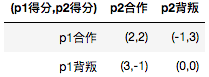
\includegraphics{intro} \\
如此連續進行N局,最後結算雙方的平均得分

\end{frame}

\begin{frame}
\frametitle{Definition(1)}

\begin{itemize}

\item 「一局」比賽將有$N$輪,其中雙方無法探知確切輪數、且非常多$N\to\infty$
\item 在第$n$輪(round)中雙方玩家$\{p_1,p_2\}$要做出決策 \\ $\{$合作,背叛$\}$$\mapsto\{1,0\}$
\item 可能agents的集合稱為「池子」
	\begin{itemize}
	\item 代號:$\{A_1,A_2,...,A_k\}$
	\item 一場捉對比賽抽到對手$A_i$的機率是$\frac{1}{k}$
	\end{itemize}

\end{itemize}

\end{frame}

\begin{frame}
\frametitle{Definition(2)}

\begin{itemize}

\item 本局比賽前n輪的狀態矩陣$\phi_n$
$$
\phi_n=\begin{bmatrix}
r_{11} & r_{12} \\
r_{21} & r_{22} \\
r_{31} & r_{32} 
\end{bmatrix}
$$
\item 當我們和Agent對局的時候我們是player1(column1)、Agent是player2(column2)\\ 每一輪Agent的反應函數記作:
$$
A_i(\phi_{n-1})=r_n=\left\{\begin{array}{lr} 1, & \text{cooperate} \\ 0, & \text{betray} \end{array} \right.
$$
\item 也就是依據前n-1局(n-1 rows)的資訊來做第n局的決策$r_n$
	\begin{itemize}
	\item 假設我們是$p_1$、agent是$p_2$來說,agent第n輪的回應就是新矩陣$\phi_n$中的$r_{n2}$值
	\end{itemize}

\end{itemize}

\end{frame}

\begin{frame}
\frametitle{Agent反應函數(1)}

\begin{itemize}

\item AgentMu 
$$
 \text{AgentMu}_\mu(\phi_{n-1})=X_\mu\text{ , }X_\mu\sim Bernoulli(\mu)
$$
\item AgentQ
	\begin{itemize}
	\item 透過$\phi_{n-1}$去估計對手可能的合作機率
	\item 第n局時,定義觀察到前n-1局對手合作的次數是m:
	$$
	m=\sum_{i=1}^{n-1} r_i^{opponent}
	$$
	\item 在完全沒有任何資訊的情況下,我們希望初始機率是$\frac{1}{2}$ \\ 於是調整估計式q為:
	$$
	\begin{aligned}
	q
	&=
	\frac{(m)+1}{(n-1)+2}
	\\
	&=
	\frac{m+1}{n+1}
	\end{aligned}
	\Rightarrow\text{AgentQ}(\phi_{n-1})=X_p\text{ , }\begin{cases}
	X_p\sim Bernoulli(p) \\
	p=q=\frac{m+1}{n+1}
	\end{cases}
	$$
	\end{itemize}

\end{itemize}

\end{frame}

\begin{frame}
\frametitle{Agent反應函數(2)}

\begin{itemize}

\item AgentGamma : 另加入保守係數$\gamma$,改寫為AgentGamma如下:
$$
0<q^\gamma<1\text{ , }0<\gamma<\infty
$$
$$
\text{AgentGamma}_\gamma(\phi_{n-1})=X_p\text{ , }\begin{cases}
X_p\sim Bernoulli(p) \\
p=q^\gamma=(\frac{m+1}{n+1})^\gamma\text{ , }0<\gamma<\infty
\end{cases}
$$

\end{itemize}

\end{frame}

\begin{frame}
\frametitle{Agent的行為}

\centering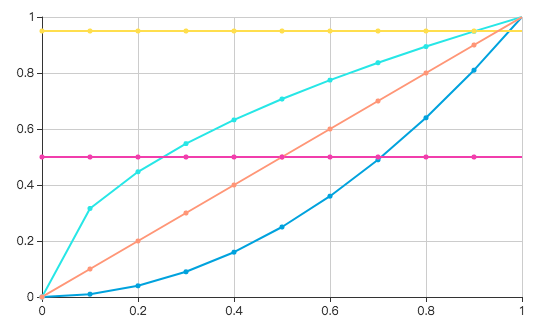
\includegraphics[width=90mm,scale=0.7]{behave}

\end{frame}

\begin{frame}
\frametitle{運用貝氏定理推算對手類型(1)}

$$
P(A_i\mid \phi_n) = \frac{\overbrace{P(\phi_n \mid A_i)}^{Likelihood}P(A_i)}{\underbrace{P(\phi_n)}_{Evidence}}
$$
已知Agent只有k種$\{A_1,A_2,...,A_k\}$ \\
其中發生對局紀錄$\phi_n$的機率$P(\phi_n)$可以由總機率法則:
\begin{small}
\[
P(A_1\mid \phi) = \frac{P(\phi \mid A_1)P(A_1)}{P(\phi\mid A_1)P(A_1)+P(\phi\mid A_2)P(A_2)+\dots+P(\phi\mid A_k)P(A_k)}
\]
\end{small}
\end{frame}

\begin{frame}
\frametitle{運用貝氏定理推算對手類型(2)}

設定每一種agent出現的機率都是$P(A_1)=P(A_2)=...=P(A_k)=\frac{1}{k}$  \\
整理後得到:
$$
P(A_1\mid \phi) = \frac{P(\phi \mid A_1)}{P(\phi\mid A_1)+P(\phi\mid A_2)+\dots+P(\phi\mid A_k)}
$$
很直覺地給定發生$\phi_n$,對手是$A_i$的機率就是Likelihood的相對比例:
$$
\frac
{Likelihood(A_i)}
{\sum_{j=1}^k Likelihood(A_j)}
$$

\end{frame}

\begin{frame}
\frametitle{計算Likelihood(AgentMu)}

方便起見以下定義$p_{n}$為第n輪心中願意合作的機率:
$$
\begin{aligned}
P(\phi_n\mid \text{AgentMu}_\mu)
&=
\prod_{n=1}^N
\begin{cases} 
p_{n}&\text{ , if }r_n~cooperate \\ 
1-p_{n}&\text{ , if }r_n~betray 
\end{cases}
\\
&=
\prod_{n=1}^N
\begin{cases} 
\mu&\text{ , if }r_n~cooperate \\ 
1-\mu&\text{ , if }r_n~betray 
\end{cases}
\because p_n=\mu
\end{aligned}
$$

\end{frame}

\begin{frame}
\frametitle{計算Likelihood(AgentGamma)}

AgentGamma在第n輪時會觀察對手合作比率$q_n$ \\
(是$\phi_n$的函數:$q_n=q_n(\phi_n)$)\\
進而依保守係數$\gamma$作指數運算得到心中願意合作的機率:
$$
p_n=q_n^\gamma
$$
$$
\begin{aligned}
P(\phi_n\mid \text{AgentGamma}_\gamma)
&=
\prod_{n=1}^N
\begin{cases} 
q_{n}^\gamma&\text{ , if }r_n~cooperate \\ 
1-q_{n}^\gamma&\text{ , if }r_n~betray 
\end{cases}
\end{aligned}
$$

\end{frame}

\begin{frame}
\frametitle{判斷對方方法:分組判斷法}

\begin{itemize}
	\item 目標:得分極大化
	\item 分成兩組:
	\begin{itemize}
		\item AgentMu 
		\begin{itemize}
			\item 永遠背叛平均得分$\rightarrow3\mu$
		\end{itemize}
		\item AgentGamma
		\begin{itemize}
			\item 永遠合作平均得分$\rightarrow2$
		\end{itemize}
	\end{itemize}
	\item 問題簡化成:
$$
P(A_{Trust}\mid \phi_n)
=
\frac
{\sum_{i\in \text{Trust}}Likelihood(A_i)}
{\sum_{j=1}^k Likelihood(A_j)}
$$
\end{itemize}

\end{frame}

\begin{frame}
\frametitle{Claim}

局數趨近無窮多,$P(A_{Trust}\mid \phi_n)$會收斂到真實的對手類型:
$$\lim_{n\to \infty}
P(A_{Trust}\mid \phi_n) = 
\begin{cases}
1\text{ , }A_{Trust} \\ 
0 \text{ , }\neg A_{Trust}
\end{cases}
$$

收斂的原因:
\begin{enumerate}
	\item 假設$AgentMu$中合作機率最大的$\mu=1-\epsilon$
	\item 若$\epsilon=0$, 只要出現一局背叛就能確定$P(A_{\mu=1}\mid \phi_n)=0$
	\item 若$0<\epsilon<1$
	\begin{itemize}
		\item 因為我們全部合作,$AgentGamma$估計的q值會往1收斂
		\item 存在$n_1$使得$n>n_1, q_n>\mu$(對所有$AgentGamma$)
		\item 此時所有$AgentGamma$的合作機率都大於$AgentMu$,局數越多越能有效區分
	\end{itemize}
\end{enumerate}

\end{frame}

\begin{frame}
\frametitle{實驗一:mu$\sim$U(0, 1), gamma$\sim$U(0.2, 1.5)}

Answer = mu
\centering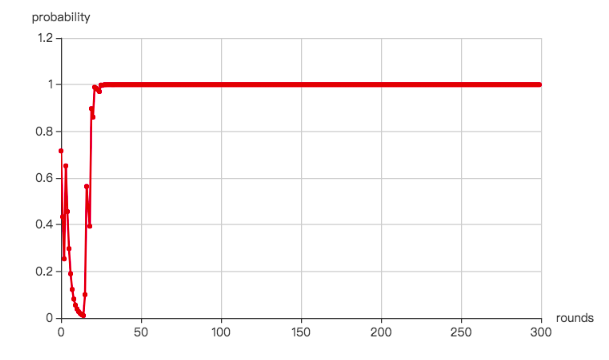
\includegraphics[width=90mm,scale=0.7]{exp1-1}

\end{frame}

\begin{frame}
\frametitle{實驗一:mu$\sim$U(0, 1), gamma$\sim$U(0.2, 1.5)}

Answer = gamma
\centering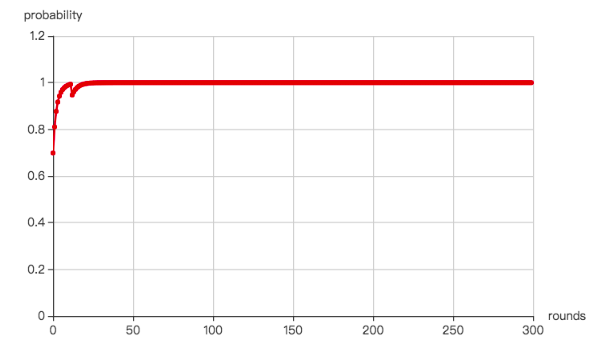
\includegraphics[width=90mm,scale=0.7]{exp1-2}

\end{frame}

\begin{frame}
\frametitle{實驗二:mu$\sim$U(0.95, 1), gamma$\sim$U(0.01, 0.1)}

Answer = mu
\centering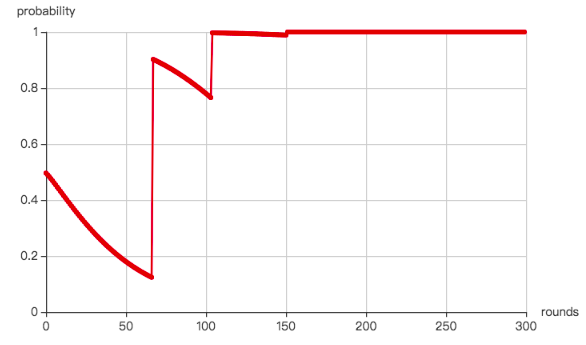
\includegraphics[width=90mm,scale=0.7]{exp2-1}

\end{frame}

\begin{frame}
\frametitle{實驗二:mu$\sim$U(0.95, 1), gamma$\sim$U(0.01, 0.1)}

Answer = gamma
\centering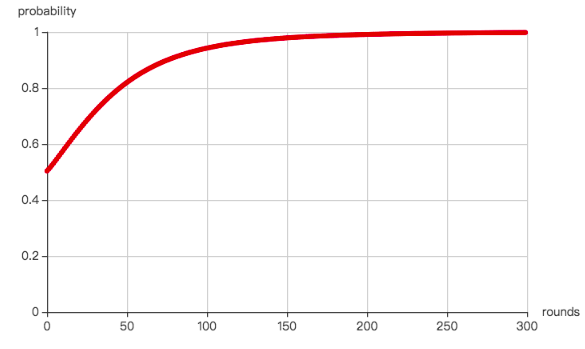
\includegraphics[width=90mm,scale=0.7]{exp2-2}

\end{frame}

\begin{frame}
\frametitle{實驗三:mu$\sim$U(0, 0.05), gamma$\sim$U(10, 20)}

Answer = mu
\centering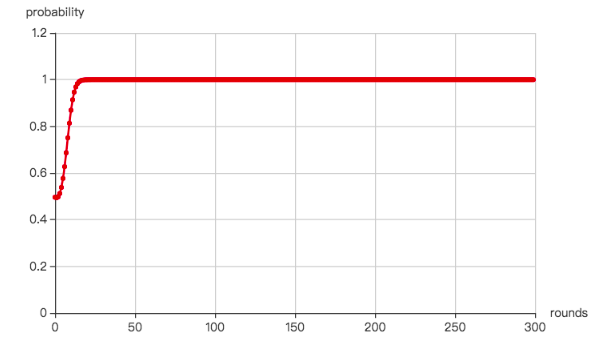
\includegraphics[width=90mm,scale=0.7]{exp3-1}

\end{frame}

\begin{frame}
\frametitle{實驗三:mu$\sim$U(0, 0.05), gamma$\sim$U(10, 20)}

Answer = gamma
\centering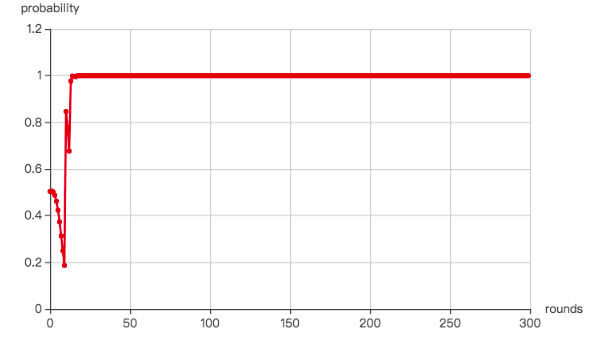
\includegraphics[width=90mm,scale=0.7]{exp3-2}

\end{frame}

\begin{frame}
\frametitle{實驗四:極端組合}

Answer = mu$\sim$U(0, 0.05)
\centering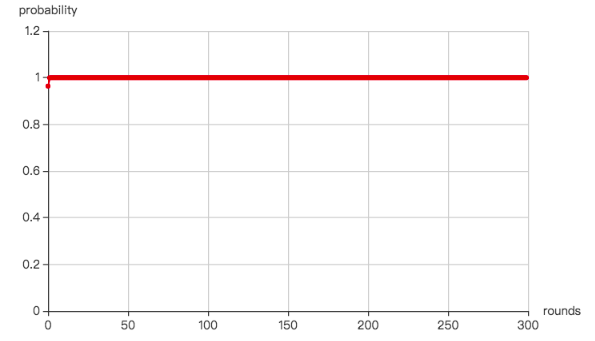
\includegraphics[width=90mm,scale=0.7]{exp4-1}

\end{frame}

\begin{frame}
\frametitle{實驗四:極端組合}

Answer = mu$\sim$U(0.95, 1)
\centering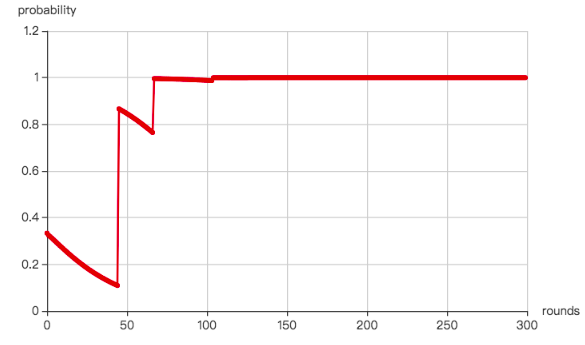
\includegraphics[width=90mm,scale=0.7]{exp4-2}

\end{frame}

\begin{frame}
\frametitle{實驗四:極端組合}

Answer = gamma$\sim$U(10, 20)
\centering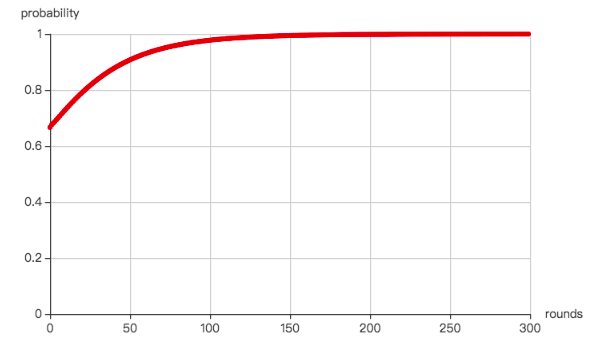
\includegraphics[width=90mm,scale=0.7]{exp4-3}

\end{frame}

\begin{frame}
\frametitle{實驗四:極端組合}

Answer = gamma$\sim$U(0.01, 0.1)
\centering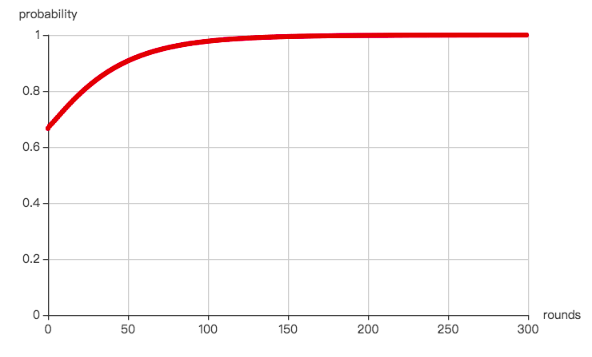
\includegraphics[width=90mm,scale=0.7]{exp4-4}

\end{frame}

\begin{frame}
\frametitle{結論}

在只有Mu,Gamma這兩種agent的情境中,最簡潔的一種高分策略是:
\begin{itemize}
	\item 1. 先全部採取合作 (stage 1)
	\item 2. 觀察對方是「不值得合作」群組的機率
	\begin{itemize}
		\item 如果該機率大於某個信心水準$\alpha$(例如0.99),從此全部採取背叛 (stage 2)
	\end{itemize}
\end{itemize}

\end{frame}

\begin{frame}
\frametitle{心靈小語}

這告訴待人處事抱持著「不主動得罪人」是有益處的,  
它讓我們可以找出值得信賴的朋友。(日久見人心)

\end{frame}

\begin{frame}

\centering 謝謝大家!

\end{frame}

\end{CJK}
\end{document}